\documentclass[12pt]{report}
\usepackage[T1]{fontenc}
\usepackage[utf8]{inputenc}
\usepackage{amsmath,amssymb,amsfonts} % Required for some math elements, equation environment and inline $ (math) $
\usepackage{makeidx}
\usepackage{graphicx} % Required for the inclusion of images
\usepackage{txfonts}
%\usepackage{times} % Uncomment to use the chosen font 
\usepackage[skip=5pt,font={small,it},labelfont=bf]{caption}
\usepackage{subcaption}
\usepackage{siunitx} % Provides the \SI{}{} and \si{} command for typesetting SI units 
\usepackage{color}
\usepackage[english]{babel} %%% SPRAWDZANIE PISOWNI EN
%\usepackage[polish]{babel} %%% SPRAWDZANIE PISOWNI PL

%%% PAGE HEADERS COMMANDS %%%
\usepackage{fancyhdr} % Page Headers and Footers
\pagestyle{fancy} %page style with FancyHDR package
\fancyhf{} % clear the header/footer style
\lhead{\leftmark} % hdr left - standard marking (chapter names)
\rhead{\thepage} % hdr right - page numbering
%\setlength{\textwidth}{14cm}
\setlength{\textheight}{20cm} 

% BIB REF COMMANDS
\usepackage[nottoc,notlot,notlof]{tocbibind}
\usepackage[backend=bibtex,style=alphabetic,sorting=anyvt]{biblatex}  
\addbibresource{references.bib}
%Bibliography sorting options 
%option	description
%nty	sort by name, title, year
%nyt	sort by name, year, title
%nyvt	sort by name, year, volume, title
%anyt	sort by alphabetic label, name, year, title
%anyvt	sort by alphabetic label, name, year, volume, title
%ydtn	sort by year (descending), name, title
%none	entries are processed in citation order

% CODE LISTINGS COMMANDS
\usepackage{verbatim} % Pre-formatted text environment 
\usepackage[linesnumbered,ruled,vlined]{algorithm2e} % Algorithms with ctan algorithm2e 
\usepackage{listings}
\definecolor{mygray}{rgb}{0.4,0.4,0.4}
\definecolor{mygreen}{rgb}{0,0.6,0.4}
\definecolor{myorange}{rgb}{0.8,0.2,0}
\lstset{ 
	basicstyle=\footnotesize\sffamily\color{black},
	keywordstyle=\color{mygreen},
	commentstyle=\color{mygray},
	identifierstyle=\color{blue},
	stringstyle=\color{myorange},
	numbers=left,
	numbersep=5pt,
	numberstyle=\tiny\color{mygray},
	frame=tbTB,
	breakatwhitespace=false,         
	breaklines=true,                 
	captionpos=t,                    
	keepspaces=true, 
	columns=fullflexible,
	showstringspaces=false,
	float=t,
	tabsize=2,
	title=\lstname,
	caption=\lstname,
	language=C++
} 


%\newtheorem{definition}{Definicja} % przykład nowego środowiska 
%\newtheorem{example}{Przykład}[chapter] % przykład nowego środowiska 
%\newtheorem{corollary}{Wniosek}[chapter] % przykład nowego środowiska 

%%% TO DO notes
\usepackage[textsize=footnotesize]{todonotes}
% \usepackage[disable]{todonotes}
\newcommand{\td}[1]{\todo[inline]{TO DO: #1}}

%%% TOC HYPERLINKS %%%
\usepackage{hyperref}
% remember to use \tableofcontents after title
\hypersetup{
	colorlinks,
	citecolor=black,
	filecolor=black,
	linkcolor=black,
	urlcolor=black,
	pdftitle={Generating two-dimensional game maps with use of cellular automata},
	bookmarks=true 
}  

%%% STRONA TYTUŁOWA - DANE
\title{Generating two-dimensional game maps with use of cellular automata}
\author{Michał Wolski}

\begin{document}

\maketitle
\tableofcontents 



%%%%%%%%%%%%%%%%%%%%%%%%%%%%%%
\chapter{Introduction} \label{rozdzial.wstep} 
During recent years, presence of computer games in human lives has increased. The demand for games has shown that playing games, both as a medium of expression and a means for entertainment, is a desirable form of activity. However, as the demand for games rises \footnote{The Interactive Software Federation of Europe compiles and publishes statistics which include frequency of gaming in European countries and show that demand for games is on the rise. \url{https://www.isfe.eu/industry-facts/statistics}} and computer games become increasingly complex, demand for game content must also rise -- game elements such as believable maps, textures, sound and models (among other types of content) are a necessary resource for production of games. Studies such as \autocite{hendrikx2013procedural} show where the evidence for insufficiency of manual content creation may be found. In the study, authors point to work of Kelly and McCabe \autocite{kelly2007citygen}, Lefebvre and Neyret \autocite{lefebvre2003pattern}, Smelik et al. 2009 \autocite{smelik2009survey} and Iosup 2009 \autocite{iosup2009poggi} as sources which reveal game content production as a time-consuming and expensive endeavour.

\subsubsection{Solving the inefficiency issue}
Scientific surveys such as \autocite{hendrikx2013procedural} and \autocite{smelik2009survey} show why investigating procedural generation is useful for the game industry, by providing examples of successful methods which can be used to generate content for games. Primary concerns which drive the interest in automated ways to create game content are the rising project costs and increasing development time.

In order to reduce the cost of game development, allow for greater replay value or provide a feeling of vastness to the game worlds that designers aim to create, procedural content generation techniques can provide an attractive solution to the problem of content creation. Surveys such as \autocite{hendrikx2013procedural}, \autocite{togelius2011search} and \autocite{de2011survey} show what types of game content can be generated and are a good starting point for seeking methods of procedural generation.

\subsubsection{Personal motivation}
During two recent years, the author of this thesis took part in a small, after-hours independent game development project. Working with a group of friends, using Unreal Engine as a tool to develop a simple prototype of a game belonging to the \textit{rogue-like} game genre. The project is still in development phase and finding a good method of map generation can potentially result in contribution of useful features.

%%%%%%%%%%%%%%%
\section{Thesis structure}
The overall structure of this thesis includes introduction followed by three chapters. The second chapter \ref{rozdzial.teoria} serves as a study on possible mechanisms that could be used for procedural generation and specifically, for creation of 2D maps for games. The chapter \ref{rozdzial.praktyka} describes performed experiments, design and implementation of a solution to the problem. Chapter \ref{rozdzial.podsumowanie} summarizes the findings and concludes the thesis, followed by chapter \ref{rozdzial.kod} which lists full source code of the developed solution.

%%%%%%%%%%%%%%%
\section{Objectives}

This work focuses on automated creation of 2-dimensional game maps using a cellular automata approach. We aim to do so by generating small map tiles, which can be later merged into a bigger map. Such approach allows for a degree of control to the map designer - who may want to decide which tiles will be merged and at which locations in the map they will be present. Moreover, we could also allow for editing the tile before placing it in the map. An approach that integrates manual editing or parametrization of desired results with procedural generation techniques has been proposed before \autocite{bidarra2010integrating}, \autocite{smelik2010integrating}, \autocite{smelik2011declarative}.

We focus on creation of maps for games, since literature shows map generation as an interesting area for experimentation, although personal motivation influenced the choice as well.

Beginning experimentation with flat maps on 2-dimensional plane avoids the complexity that may arise when dealing with higher dimensions.

We will investigate existing methods for procedural generation of game maps which resemble cave structures. Then, an approach that may be used for automated creation of such maps will be selected and examined with a focus on implementing a working map generator. Main points of focus for this project are as follows:

\begin{itemize}
	\item research on procedural generation of maps
	\item selecting a promising approach to use
	\item designing a map generator program
	\item implementing the solution in a programming language of choice
\end{itemize}

\td{Objectives - is that all?}

%%%%%%%%%%%%%%%
\section{Thesis scope}

\td{scope - what we will do and what we will not }

\td{scope }

\td{scope - shortly: what could be done instead}

%%%%%%%%%%%%%%%
\section{Technology and tools}

The following paragraphs summarize what tools were involved during the project of thesis preparation and performing the experiments.

\subsection{Hardware} 

All experiments in this thesis have been performed using a laptop with an {Intel Core i7 2630QM - x64 2.0 \si{GHz}} multi-core processor, {16GB RAM} and an {nVidia GeForce GTX 560M} graphics card.
 
\subsection{Software} 

Development environment for the purposes of thesis experiments and writing has been set up under Windows 10 operating system with the following software installed:

\begin{itemize}
	\item Visual Studio 2015 Community IDE
	\item CMake for Windows
	\item TeXstudio editor with MikTeX back-end
	\item Git version control system
	\item Notepad++
	\item UMLet open source modelling program
	\item \td{...}
\end{itemize}

Other configuration details include: \td{environment variables, configuration specifics...} 

This thesis has been prepared with \LaTeX\space system for document typesetting.

 
\subsubsection{Programming languages} 

The program that allowed to carry out experiments in this thesis was implemented using the C++ programming language and compiled with MSVC++ 14.0 compiler, natively included in the VS2015 IDE.  

\subsubsection{Libraries} 

The implementation uses following libraries:
\begin{itemize}
	\item Dear ImGui, by Omar Cornut - to easily build an Immediate Mode user interface. Project homepage:  \url{https://github.com/ocornut/imgui}
	\item GLFW 3.2.1 library - to create an OpenGL context and have direct access to texture functions. Project homepage: \url{http://www.glfw.org/}
	\item \td{...} 
\end{itemize}  
 

\subsection{Other tools }
\subsubsection{Design patterns} 
\td{list used design patters, if any. Singleton? Command? Factory?}
 


%%%%%%%%%%%%%%%
\section{Related work (?)} 

\td{think what could be included here}

%%%%%%%%%%%%%%%%%%%%%%%%%%%%%%
\chapter{Research on 2D map generation methods} \label{rozdzial.teoria}

%%%%%%%%%%%%%%%
\section{Maps and cartography} 

Historically, maps have been used by the human race since ancient times. The need for navigation in the world has been a driving force behind the evolution of maps. Starting with cave paintings and representations of stars on the sky, our kind had the need for capturing an abstract model of a territory, terrain shape, location of useful resources or some other aspect of surrounding environment in a useful way.

Making a model of the physical (or fictional) world with maps requires choice of the data types describing locations represented on the map. List of data types visualized with maps has been growing with the evolution of cartography and whenever new technologies have been introduced to the map making crafts. Some examples of data possible to represent on maps are:
 
\begin{itemize}
	\item physical maps - terrain shape, elevation, forests, bodies of water, etc.
	\item political maps - borders around a territory, districts, states
	\item climate and weather maps - temperature, humidity, precipitation, wind currents
	\item geologic maps - terrain features, location of precious resources underground
	\item star maps - views of the distant cosmic objects measured by solid angles from a fixed point
	\item route maps - transport links, connections joining points on the modelled territory
\end{itemize}

Although early maps had the form of drawings or etchings on surface of solid materials, now there are other possibilities of representing the abstract model which a map aims to represent. The rise of digital maps and geographic information systems has opened new possibilities - maps have become dynamic entities, stored digitally, easily updated with new data and not limited to the boundaries of physical model. With digital maps, it is possible to show more than one layer of data, as chosen by the user, whereas physical maps are limited to the data and view scale chosen initially at the time when map was crafted. Despite the limitations, they still can serve well as a medium for storage of geographic information, requiring simpler processes during archival and conservation efforts. Deeper exploration into the subject can be found in Bagrow's History of Maps \autocite{bagrow2017history}.

\begin{figure}[h!]
	\centering
	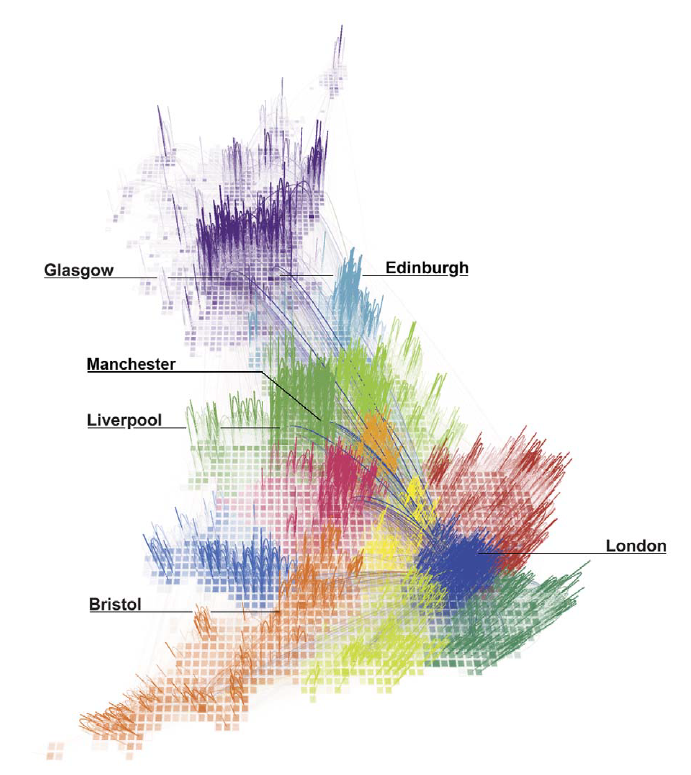
\includegraphics[width=0.6\linewidth]{images/journal_netw_talk_map}
	\caption{Pure data map showing the geography of talk in Great Britain. Authors measured the total talk time via communication networks between areas in Britain and used the data to produce the visualzation. Source article: \autocite{10.1371/journal.pone.0014248}}
	\label{fig:journalnetwtalkmap}
\end{figure}


Digital technology has also brought interesting methods to the art of crafting maps, allowing for new types of maps to be crafted, which brought previously undiscovered insights into the nature of represented territories. For example, with data maps such as the one described by article 'Redrawing the Map of Great Britain from a Network of Human Interactions' \autocite{10.1371/journal.pone.0014248} it is possible to draw more useful borders around regions, fitting actual human interaction groups as opposed to those defined by past governments. Authors of the article present a visualization of the data, which has a map form - see figure \ref{fig:journalnetwtalkmap}.

The possibility of visualizing map layers which could not have been created and shown without digital data processing techniques and ease of experimentation with the information and algorithms used to create modern digital maps have also made it apparent that the source data for the layer itself do not necessarily have to measure some aspect of reality, but can be generated using mathematical methods. Such approach effectively allows for creation of fictional maps, representing imaginary territories. With that in mind, let us now move on to the sphere of fictional maps and their use in games, physical and digital alike. 


%%%%%%%%%%%%%%%
\section{Maps in games} 

It is not clear what kind of game was the first one in history to use a map to represent the game world, however two notable examples may easily come into mind: Chess and Go, which are both widely known around the world. 

Chess, a board tactical war-game developed before 6th century AD, uses black-white board as the map of its world. Although the environment represented by a chess board is very simple, it has some important features and rules. The map is composed of square cells, which are arranged on 8 by 8 grid, effectively creating a rigid boundary around the game world, which according to game rules - cannot be crossed. Each cell has 8 neighbours and can be occupied by only one game piece.

Another game, originating from ancient China, defines a similar, grid-based game world, effectively making a map of a uniform planar territory. Go is played on 19 by 19 board, however smaller board sizes are used as well. In Go, the goal is to capture more territory than the opponent, which is done by placing game pieces on line intersections, one piece per turn.

\td{expand on Go, comment on both, then introduce modern board games}


\begin{figure}[h]
	\centering
	\begin{subfigure}[b]{0.4\linewidth}
		\centering
		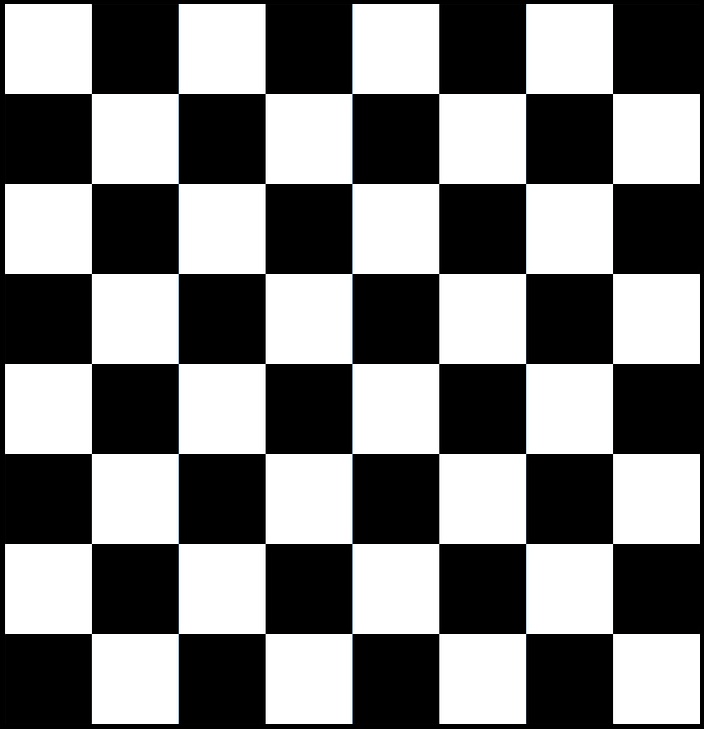
\includegraphics[width=\textwidth]{images/chessboard}
		\caption{Chess board} 
	\end{subfigure}
	\hfill
	\begin{subfigure}[b]{0.4\linewidth}
		\centering
		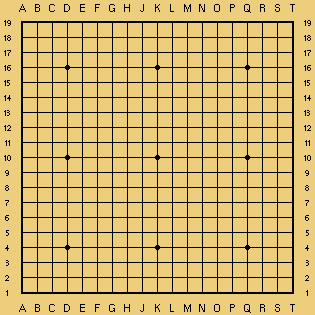
\includegraphics[width=\textwidth]{images/goboard}
		\caption{Go board} 
	\end{subfigure} 
	\caption{Chess and Go both use planar boards divided into tiles by a square grid - simple maps to represent the environment in which game is played.}
	\label{fig:neighborhood_types}
\end{figure}
 
Another interesting example of a game world map is the multi-player strategy board game Risk, invented in 1957 by Albert Lamorisse, where the map represents a territory divided into regions, which must be captured by players in order to win. Risk game shows how a political world map with imagined region borders can be creatively used in a game, as a resource for the players to fight over. The game of Risk has been since published in many variations. Most of them share the same gameplay goal: to capture more territory than the opponents do, which is an example of how a game might use environments represented by maps as a limited resource for players to acquire.
 
\begin{figure}[h]
	\centering
	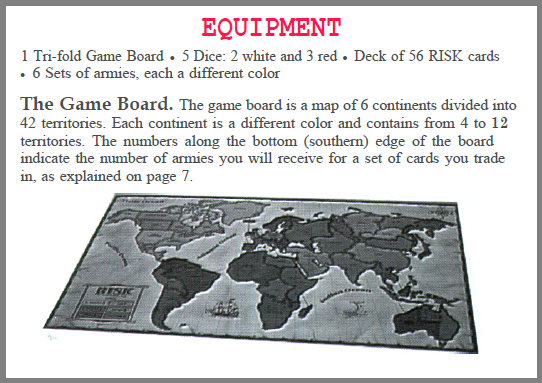
\includegraphics[width=0.5\linewidth]{images/risk-rulebook} 
	\caption{Risk rule book fragment, containing a photo of the game board. The board shows a world map with fictional political borders, dividing the map into regions, which serve as a resource for players to capture. Image source: photo taken from original Risk rule book, copyright Hasbro 1993}
	\label{fig:acrord32risk1}
\end{figure}

Modern board games have introduced many new ideas to the design of game boards. One example of such ideas is bringing modularity into the board design, composing pieces of the board similarly to how a jigsaw puzzle is composed of singular pieces. Such arrangement allows for greater value in replaying the game, since the game world can be different at each time the game is played. 

An example of such game is Carcassonne, published in 2000, designed by Klaus-Jürgen Wrede in Germany. The game of Carcassonne involves an interesting mechanism: rather than having a fixed game board, cards with tiles are used to construct the board during gameplay. The game rules around tile placement can be thought of as an algorithm of procedural generation: only one tile can be placed during each game turn, adjacent to other tiles, forming a connection with features that tiles represent - roads must connect to roads, fields to other fields, and cities to cities. The rules ensure that the players will develop the game board as the game progresses, which leads to an interesting observation: each turn, the players are presented with new territory to consider in their decisions - and since the game requires players to deploy their resources onto the constructed game map in order to accumulate score and eventually win, these decisions may often become quite challenging with increasing complexity of the board layout.

\begin{figure}[h]
	\centering
	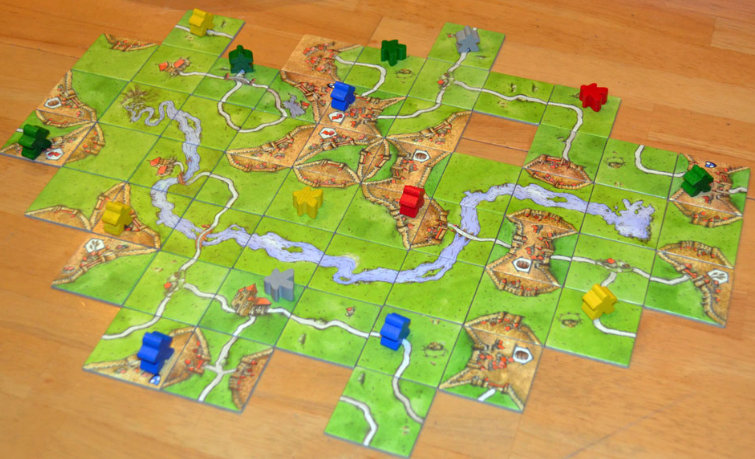
\includegraphics[width=0.7\linewidth]{images/carcassonne}
	\caption{Carcassonne game board during gameplay. Players place tiles adjacent to existing ones, making sure that each tile fits the others. Image source: https://deerfieldlibrary.org/2016/01/carcassonne-a-modern-board-game-for-adults-teens/}
	\label{fig:carcassonne}
\end{figure}


\td{comment - board games: map creation mechanics, rules}
\td{carcassone web version at https://concarneau.herokuapp.com/game}

However, some of the more complex game rules and ideas are better implemented using computer simulation, since most of the mundane tasks which do not contribute to gameplay can be automated. Random number generation, board preparation and arrangement, checking player moves against game rules - all those activities are good candidates for automation. The other reason to simulate games may be to develop artificial intelligence algorithms which can simulate player behaviour at a chosen level of competitive play, effectively providing a way for beginners who want to learn the game they are interested in or for veterans who want to develop their skills further, as has been done for chess and other classic board games.
 
There are many more examples of modern board games which involve interesting mechanics, but their description lies beyond the scope of this thesis project. Moving on, we will now investigate a few examples of computer games and simulations, where maps are used to construct some aspects of gameplay.
%%%%%%%%%%%%%%%
\section{ Interactivity }

The evolution of personal computers has allowed players to enjoy a new form of entertainment - video and computer games. Possibility of performing real-time simulations on computers and development of computer graphics rendering techniques have created a new medium of expression in the form of computer software. At the time when early forms of interactive simulations were created, first computer games were also developed. Examples like 




\td{examples from games: Diablo, NetHack (1987), Ultima Ratio Regum, Dwarf Fortress (2006), }
\td{\url{http://www.roguebasin.com/index.php?title=Major_roguelikes}}
\td{http://ascii-patrol.com/map.png + source?}

\begin{figure}[h]
	\centering
	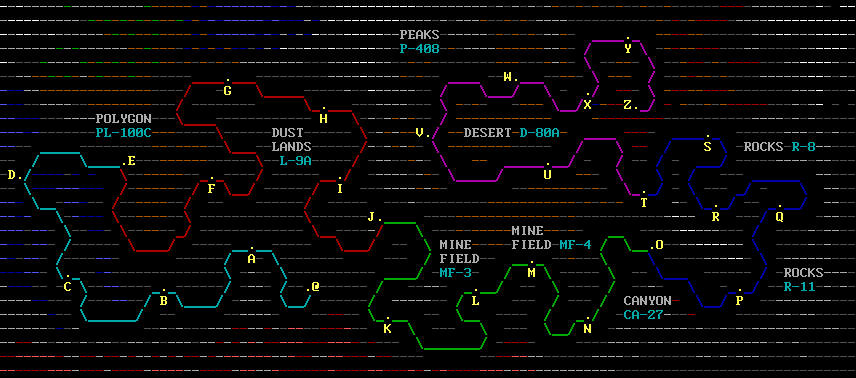
\includegraphics[width=0.9\linewidth]{images/map}
	\caption{A game map using ASCII art}
	
	\label{fig:map}
\end{figure}
\todo{find out what game ascii art map is from}

%%%%%%%%%%%%%%%
\section{ Automation - reduction in development time and cost}

As stated in chapter \ref{rozdzial.wstep}, our context does not deal with projections of 3D objects onto a plane, like the fields of geography and cartography do \autocite{snyder1993flattening}. Our goal is simply to generate planar maps. 


\td{ write about PCG in general, short }
\td{ PCG types of content }
\td{ PCG methods }
\td{ focus on maps }
 



%%%%%%%%%%%%%%%
\section{Existing solutions for 2D map generation}

In scientific surveys on PCG methods, we find approaches to map generation employed in the past. As listed by Hendrikx et al. \autocite{hendrikx2013procedural}, \td{list map procgen methods}

\td{HOW it was done until now? options?}
\td{ ref survey with table of 2d dungeon gen}

\subsection{Cellular automata}

A cellular automaton is a simulation in which every object in a mathematically defined space is being updated at every step of a simulation. Historically, cellular automata and their properties have been studied since the time of first electronic computers \autocite{Sarkar:2000:BHC:349194.349202}. One of the most complete sources on cellular automata is a book summarizing research on CA carried out by Stephen Wolfram since 1980s \autocite{wolfram2002new}, where a classification of cellular automata is shown along with examples for each kind of CA. 

Specifically, 2-dimensional automata operate on a grid of cells with arbitrary discrete dimensions. Each cell in the grid has neighbours, which may be relevant to the simulation rules. Depending on the type of rules which are used by a particular CA, a different type of cell neighbourhood may be used. To present this concept concisely, a short list of definitions follows.

\begin{description}
	\item[Cell] A cell is simply one unit positioned in CA simulation space. Cells have state, which can be simple  - for example, a binary digit, an integer - or more complicated - a real number with constraints, a complex number, or other.  
	\item[Cell neighborhood] In a context of a 2D square grid of cells, neighbourhood is a collection of nearest cells to the selected one.
	\item[Moore's neighbourhood]  Moore neighbourhood includes the cell and its immediate neighbours - one to the north, south, east and west of the cell, as shown in figure \ref{fig:neighborhood_types}.
	\item[Von Neumann neighbourhood] Von Neumann neighbourhood includes 8 closest neighbours of the cell - immediate and diagonal, as shown in figure \ref{fig:neighborhood_types}.
	\item[Other types of neighborhood] It is possible to imagine other types of cell neighbourhoods, possibly including more cell rings around a cell or only a selection of them arranged in a custom pattern. Those cases are beyond the scope of this thesis.
\end{description}
 
\begin{figure}[h]
	\centering
	\begin{subfigure}[b]{0.35\textwidth}
		\centering
		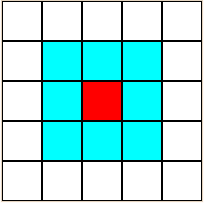
\includegraphics[width=\textwidth]{images/neighborsmoore}
		\caption{Moore neighborhood} 
	\end{subfigure}
	\hfill
	\begin{subfigure}[b]{0.35\textwidth}
		\centering
		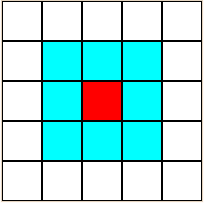
\includegraphics[width=\textwidth]{images/neighborsvonneumann}
		\caption{Von Neumann neighborhood} 
	\end{subfigure} 
	\caption{Two basic types of cell neighborhood}
	\label{fig:neighborhood_types}
\end{figure}


There are ...

Every CA simulation also consists of rules which drive the process of cell evolution to its next stage. Typically, such rules define how board elements must be changed once a specific element arrangement is recognized.

\td{ca basics - game of life}
\td{using CA for simulations }
\td{using CA for generation of content}



\subsection{Generative grammars}

\td{Sportelli, Francesco \& Toto, Giuseppe \& Vessio, Gennaro. (2014). A Probabilistic Grammar for Procedural Content Generation. 10.13140/2.1.3820.4163. }
\subsection{L-systems} 

\subsection{...}

\subsection{Other methods}


%%%%%%%%%%%%%%%
\section{Choosing a method of generation}

In order to effectively judge the value that a working map generator may bring to a game development project, we need to consider what characteristics should be evaluated. First, a useful generator must be effective at map generation.

\td{how to measure effectiveness? time of map generation, map shape, desirable map features?}

Another point to consider is how easy to use such generator can be. Game designers may ultimately decide to use manual methods of map creation if the method of map generation requires too much effort to include in their project.

\td{how to measure such ease of use? accessibility? }

The third aspect of choice what a generation method could be used is to consider how much value it brings to the designer versus what development costs it can reduce.

\td{how to measure cost?}

The following subsections describe how each of the mentioned aspects can influence the choice of a generation method.

\subsection{Effectiveness} 
\td{study on generation time}
\td{desired characteristics of generated content?}

\subsection{Accessibility} 

\td{study on what makes generation easy to include in game development projects}
\td{integrating manual editing AND procgen}

\subsection{Cost} 
\td{examples of development costs - human resources, machine resources}
\td{which of these costs can be reduced by PCG}




%%%%%%%%%%%%%%%
\section{Chosen approach: cellular automata for 2D map generation}

One of possible proposed approaches is the work of L. Johnson, G. Yannakakis and J. Togelius from IT University of Copenhagen \autocite{johnson2010cellular}. 

Authors describe rules of a cellular automaton which are able to transform a tile filled initially with random distribution of cells into a tile which has interesting properties for a map designer.

\td{authors describe a process - 1 random image 2 apply CA steps as in article cave gen 3 merge tiles, result: maps!} 

\td{short paragraph on the choice of CA for game maps}
\td{why we chose CA for mapgen?}
\td{what are pros and cons of such choice?}


%%%%%%%%%%%%%%%%%%%%%%%%%%%%%%%%%%%%%%%%%%%%%%%%%%%%%%%%%%%%%%%%%%%%%%%%%%%%%%% 
\chapter{Generating and visualizing maps - proposed solution} \label{rozdzial.praktyka} 
%%%%%%%%%%%%%%%%%%%%%%%%%%%%%%%%%%%%%%%%%%%%%%%%%%%%%%%%%%%%%%%%%%%%%%%%%%%%%%% 

To describe the developed solution concisely, this chapter consists of five sections: definition of required features, design of simple CA simulation and map generator models, followed by implementing them in C++ programming language, experiments and finally, tests.

%%%%%%%%%%%%%%%
\section{Analysis of requirements for a map generator}

Having gathered the abstract constructs needed to build a CA map generator in chapter \ref{rozdzial.teoria}, we may proceed to state the requirements formally. In the following sections, we will: 
\begin{itemize}
	\item define features required of a map generator program to automate creating maps,
	\item state the desired properties of such generator,
	\item discover to what constraints such program may be required to conform.
\end{itemize}

\subsection{Functional requirements}

First, we must define the desired functions which a useful map generator must provide to its user.
Since we have selected an approach to map generation based on cellular automata in chapter \ref{rozdzial.teoria}, we have to include simulation of CA states. As described in \autocite{johnson2010cellular}, our approach consists of generating a random image, which after several transformations performed by CA rules becomes structured with island-like features. Such image can then be used as a tile for larger maps. Showing each step of image transformation could be useful to the designer, allowing them to control what kind of generated tiles will be chosen to compose the map. 

Another potentially useful feature would be manual editing of tiles before they are placed in the map, which would allow for an even greater degree of control over tile contents. Further expansion of such feature could be to provide the designer with tools to make their own rules for tile generation, while also allowing them to define types of single cells composing the tile.

Finally, a map generator without a mechanism for saving the work done by a designer would certainly not be a useful tool. Such program needs a way to export generated maps to a file format that later can be used by a game engine of choice, possibly with procedures written by other programmers. Although saving or exporting maps is not really necessary for experimentation and testing, a production version of the program should have such functionality.

To summarize desired functions of a map generator program, a list follows:
\begin{enumerate}
	\item The program must implement a cellular automaton to generate map tiles
	\item The program must show generation stages graphically
	\item The program must allow building maps from components (tiles)
	\item The program may allow manual editing of map tiles
	\item The program should have a mechanism for exporting generated maps
	\item \td{expand desired functions}
\end{enumerate}

\subsection{Non-functional requirements}

\td{nf-req intro}
\begin{enumerate}
	\item The program must have a graphical user interface.
	\item The GUI must allow to change generation parameters, which should be grouped and ordered. 
	\item The program must be responsive to user input and avoid crashing.
	\item \td{}
\end{enumerate}

\subsection{Constraints}

\begin{enumerate}
	\item Map tile generation time must not exceed 5 seconds.
	\item User interface elements must not invoke non-existent mechanisms.
	\item 
\end{enumerate}

%%%%%%%%%%%%%%%
\section{Design}
\subsection{Data structures and persistence}

\td{ how do we store data?}
\td{ diagrams of cell, board}
\td{ exporting data from generator? }
\td{ how designers can get a complete map model? } 

\subsection{Application logic} 

\td{how a generator will work}
\td{behavior diagrams}

\subsection{User interface}

\td{OpenGL immediate mode paradigm}
\td{imgui immediate mode user interface library}

\begin{figure}[h]
	\centering
	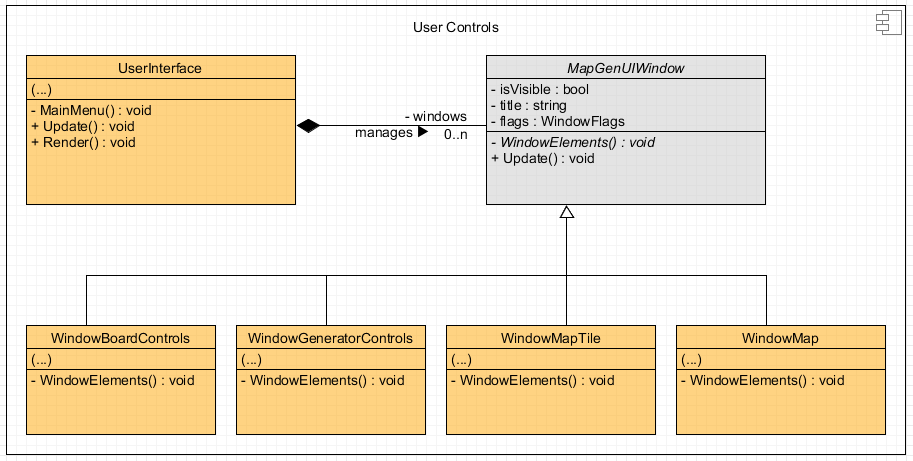
\includegraphics[width=0.8\linewidth]{diagrams/uiwindows}
	\caption[User Interface model]{Example model of classes to be used to construct user interface in the map generator program}
	\label{fig:uiwindows}
\end{figure}

\td{diagram of texture class, used by Component MapGen, uses OpenGL}

\td{mention Bret Victor talks - why we choose Immediate Mode}


%%%%%%%%%%%%%%%
\section{Basic cellular automata simulations}

Having chosen cellular automata as a method for generating maps, we need to have a clear idea about how to approach building a program that could simulate a cellular automaton. One of the helpful resources on the topic of building cellular automata simulations is chapter 7 in Nature of Code, a book by Daniel Shiffman \autocite{shiffman2012nature}, where we can find a short tutorial to build our first CA simulation. There, author describes elementary concepts needed to construct a basic CA, explains how to implement a working simulation and provides helpful exercises. The tutorial is quite useful as a guide, since examples presented in New Kind of Science \autocite{wolfram2002new} are implemented in the Wolfram language and would require familiarity with it. As stated in Nature of Code \autocite{shiffman2012nature}, a 2-dimensional CA would need the following key elements to be simulated:

\begin{itemize}
	\item Cell state - every cell has a state updated on each simulation step,
	\item Grid - a space on which cells are placed,
	\item Neighbourhood - each cell needs to know the state of its neighbours to update its state.
\end{itemize}

In order to represent the cells of an automaton, a primitive data type is sufficient. However, we could design a class which will act as a collection of cells and provide additional utility to its user. Figure \ref{fig:boardcell} presents an example model of a class that would encapsulate a collection of cell states while also preserving information about the board on which those cells are placed. 

\begin{figure}[h]
	\centering
	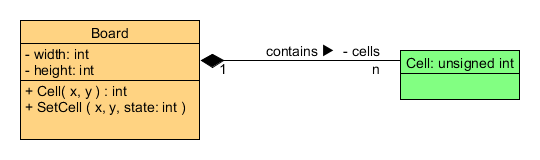
\includegraphics[width=0.8\linewidth]{diagrams/boardcell01}
	\caption{ A possible model of a Board Class which holds cell states in its block of memory and lets its user change their states} 
	\label{fig:boardcell}
\end{figure}

We can also assign a number to each cell \td{why?} as shown in table \ref{tab:cellneighbors}.

\begin{table}[h]
	\centering
	\begin{tabular}{| l | l | l |}
		\hline 
		0 & 1 & 2 \\
		\hline
		7 & S & 3 \\
		\hline
		6 & 5 & 4 \\ 
		\hline
	\end{tabular}
	\caption{Cell neighbours, numbered. \textit{S} denotes selected cell. Cells marked with odd numbers are members of Moore neighborhood of selected cell and all numbered cells are members of Von Neumann neighbourhood of it. }
	\label{tab:cellneighbors}
\end{table}


Such abstraction creates an easy to use interface for further development and is also sufficient to access the values of neighbors to the selected cell. However, in some CA simulations summing the values of cells in neighbourhood is a common operation, so we can include variations of it for convenience. Similarly, a method to translate cell states into texture points would be welcome, since we may possibly need a way to display the state of CA board on screen. Adding those elements to our abstraction yields a class presented on figure \ref{fig:boardcell2}.
 
 \begin{figure}[h]
 	\centering
 	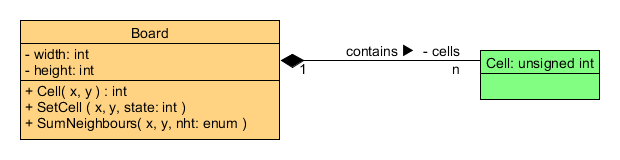
\includegraphics[width=0.8\linewidth]{diagrams/boardcell02}
 	\caption{ Revised Board abstraction - added methods for neighbor sums and translation of cell states to texels} 
 	\label{fig:boardcell2}
 \end{figure}

\td{add neighbor methods to board2}
\td{result of what it all does?}

At this point, we could also observe a common property of cellular automata  - whenever cell states need to change (the simulation moves to a later step), the state change is applied to every cell in the grid before simulation step ends \autocite{wolfram1984cellular} and cells do not need to be updated in sequence if only all cells will be changed before the next step. Hence, cell state updates could be applied in parallel to reduce the time needed to compute the simulation step. One way to do so would be to apply the findings presented by Reno Fourie in his thesis about applying CUDA technology to reduce time to compute next state of the board in case of 2-dimensional cellular automata \autocite{fourie2015parallel}.

\td{what else to include?}
\td{more on CA, 2dim CA?}


%%%%%%%%%%%%%%%
\section{Generating maps with CA}

Since the goal of this work is not to just implement a working cellular automaton simulation, we need to find a way to generate maps using CA simulation. 

\begin{figure}[h]
	\centering
	\begin{subfigure}[b]{0.2\textwidth}
		\centering
		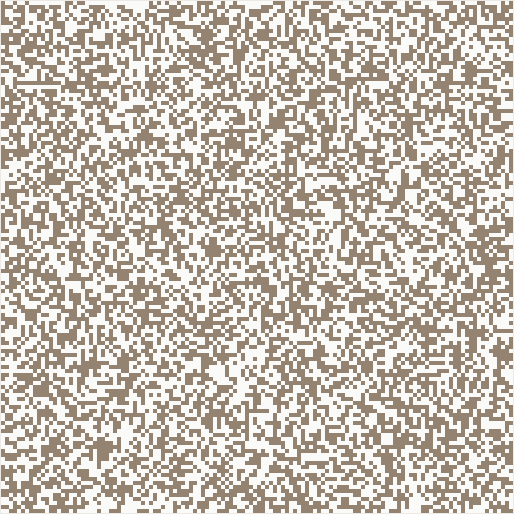
\includegraphics[width=\textwidth]{images/step1}
		\caption{Step 1 - random noise} 
	\end{subfigure}
	\hfill
	\begin{subfigure}[b]{0.2\textwidth}
		\centering
		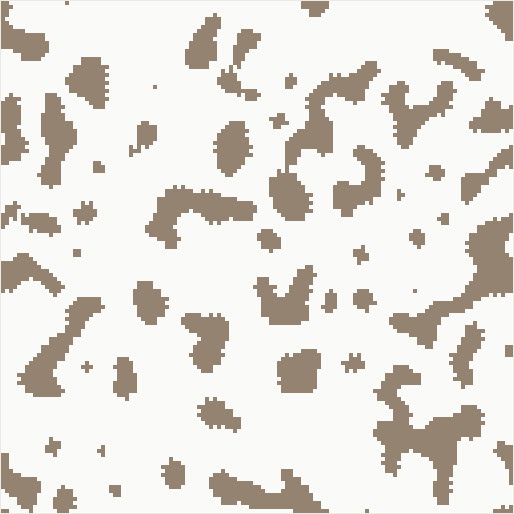
\includegraphics[width=\textwidth]{images/step2}
		\caption{Step 2 - generated tile} 
	\end{subfigure}
	\hfill
	\begin{subfigure}[b]{0.2\textwidth}
		\centering
		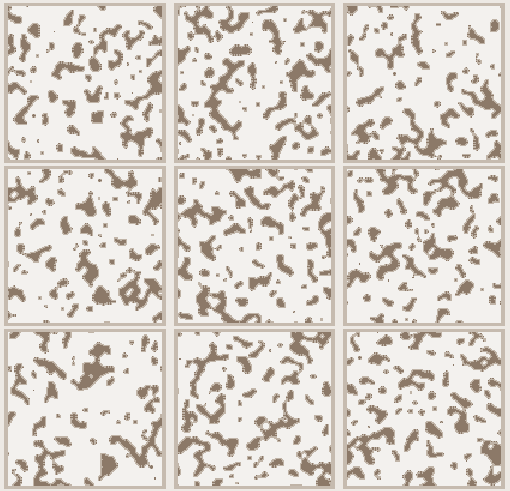
\includegraphics[width=\textwidth]{images/step3}
		\caption{Step 3 - tiles in a grid} 
	\end{subfigure}
	\hfill
	\begin{subfigure}[b]{0.2\textwidth}
		\centering
		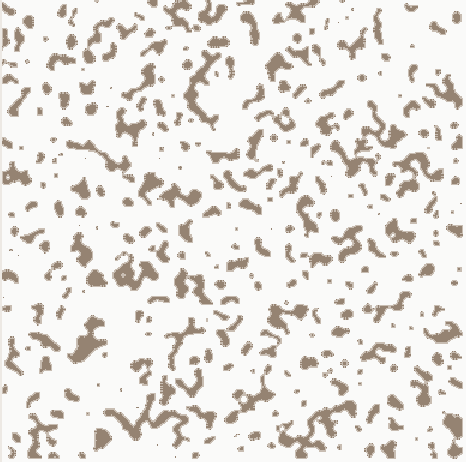
\includegraphics[width=\textwidth]{images/step4}
		\caption{Step 4 - complete map} 
	\end{subfigure}
	\caption{Four stages of map construction}
	\label{fig:map_steps}
\end{figure}






%%%%%%%%%%%%%%%
\section{Implementation}

\td{describe how it all works now, with object diagrams}
\td{refer to code itself}


%%%%%%%%%%%%%%%
\section{Tests} 

\subsection{Performance test}

%%%%%%%%%%%%%%%
\section{Deployment (?)} 

%%%%%%%%%%%%%%%%%%%%%%%%%%%%%%
\chapter{Conclusions} \label{rozdzial.podsumowanie}

%%%%%%%%%%%%%%%
\section{Evaluation of results} 

\subsection{Effectiveness}
\subsection{Accessibility}
\subsection{Cost}

%%%%%%%%%%%%%%%
\section{Perspectives for usage }

\td{map generator will be used in game project codenamed 'UW'}

%%%%%%%%%%%%%%%
\section{Further work}

\td{future: expanding the generator}
\td{future: adding more rules}
\td{future: user defined cell types}
\td{future: non-discrete cell states or more complex cell types }
\td{future: 3d maps?}

%%%%%%%%%%%%%%%%%%%%%%%%%%%%%%
%%% KONIEC PRACY %%%%%%%%%%%%%
%%%%%%%%%%%%%%%%%%%%%%%%%%%%%%
\printbibliography[heading=bibintoc]

\addcontentsline{toc}{chapter}{List of figures} 
\listoffigures

\addcontentsline{toc}{chapter}{List of tables} 
\listoftables

\addcontentsline{toc}{chapter}{List of abbreviations and acronyms} 
%%%%%%%%%%%%%%%
\chapter*{List of abbreviations and acronyms} 

The following terms, abbreviations and acronyms have been used in the thesis.

\begin{description}
	\item[CA] Cellular Automaton. A simulation consisting of cell objects.
	\item[PCG] Procedural Content Generation. An automated process of creation.   
	\item[GUI] Graphical User Interface
\end{description}
\td{(?)}  

\addcontentsline{toc}{chapter}{Attachments} 
%%%%%%%%%%%%%%%%%%%%%%%%%%%%%%
\chapter*{Attachments}
\begin{enumerate} 
\item \td{include thesis defence documents}
\item \td{?}
\item \td{?}
\item \td{?}
\end{enumerate}

\pagebreak
\listoftodos

\end{document}
